\documentclass{beamer}
\usepackage[utf8]{inputenc}
\usepackage[T1]{fontenc}
\usepackage{lmodern}
\usepackage{siunitx}

%Modifie la forme du pdf de sortie
\def\timer{0}             % 0-> sans timer     
                          % 1-> avec timer
\def\correction{1}        % 0-> sans correction après chaque question 
                          % 1-> avec correction après chaque question
                        

\usepackage{tikz}
\usepackage{xintexpr}
\usepackage{pifont}


\newcommand{\questionflash}[3]
{
\ifnum \timer=1 
\begin{frame}
\transduration{1}
\def\facteur{\xintfloateval{0.875/#2}}
\foreach \x in {0,...,#2}{\only<+>{
\textbf{Question \insertframenumber{}} 
#1    \pgfdeclarehorizontalshading{myshade}{1em}{%
         color(0\textwidth)=(rgb:green,50;-green,\x;red,\x);
        color(\x*\facteur\textwidth)=(rgb:green,50;-green,\x;red,\x);     
        color(0.1\textwidth+\x*\facteur\textwidth)=(white);
      color(\textwidth)=(white)
    }
    \begin{pgfpicture}{0pt}{0pt}{\textwidth}{1em}
        \pgfpathrectangle{\pgfpointorigin}{\pgfpoint{\textwidth}{1em}}
    \pgfusepath{clip}
    \pgftext[left,base]{\pgfuseshading{myshade}}
    \pgftext[x=.9\textwidth,y=0.5em] {\x s / #2 s}
  \end{pgfpicture}
}}
\end{frame}
 \else 
\begin{frame}
\textbf{Question \insertframenumber{}} 
#1
\end{frame} 
\fi

\ifnum \correction=1
\addtocounter{framenumber}{-1} 
\begin{frame}
\begin{center}
\textit{Correction de la question \insertframenumber{}}
\end{center}
#3
\end{frame}
\fi
}

\newcommand{\titre}[1]{
\begin{frame}\begin{center}
 \Large #1
\end{center}\end{frame}
\addtocounter{framenumber}{-1} 
\ifnum \timer=1
\begin{frame} \transduration{1} \centerline{\fontsize{200}{200}\selectfont \ding{206}} \end{frame}
\begin{frame} \transduration{1} \centerline{\fontsize{200}{200}\selectfont \ding{205}} \end{frame}
\begin{frame} \transduration{1} \centerline{\fontsize{200}{200}\selectfont \ding{204}} \end{frame}
\begin{frame} \transduration{1} \centerline{\fontsize{200}{200}\selectfont \ding{203}} \end{frame}
\begin{frame} \transduration{1} \centerline{\fontsize{200}{200}\selectfont \ding{202}} \end{frame}
\begin{frame} \transduration{1} \centerline{\fontsize{200}{200}\selectfont Go !} \end{frame}
\addtocounter{framenumber}{-6} \fi
}


 \newenvironment{quizz}[1]
 {\titre{#1}}
 {\ifnum \timer=1 \begin{frame}
Fin du quizz
\end{frame} \fi} 




   %Modifier cette ligne si qflash.tex se trouve à un autre endroit

\begin{document}
\begin{quizz}{Exemple d'utilisation de $qflash$}  %titre du quizz

\questionflash
{ %Question:
\\ $0,9999...=1 $ ?
\begin{enumerate}[a.]
\item OUI
\item NON
\end{enumerate}} 
{ %Durée d'affichage de la question:
5 }
{ %Correction 
\textbf{OUI}
\\En effet: $10 \times 0,999...=9,999... = 9+0,999...$
\\On a donc: $9 \times 0,999... = 9$ d'où $0,999...=1$.
}
\questionflash{
\begin{center}
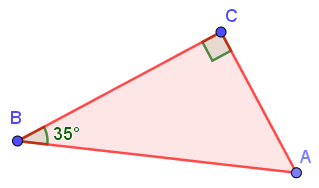
\includegraphics[scale=1]{figure.png}
\end{center}
Quelle est la mesure de l'angle $\widehat{BAC}$ ?
\begin{enumerate}[a.]
\item $\ang{145}$ 
\item $\ang{55}$
\item $\ang{65}$
\end{enumerate}
}{5}
{\begin{center}
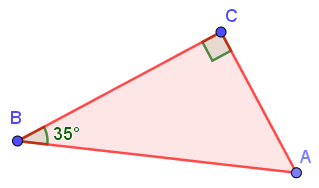
\includegraphics[scale=0.6]{figure.png}
\end{center}
\textbf{Réponse b:}
\\On utilise la somme des angles d'un triangle: 
\[ \widehat{BAC} = \ang{180}-\ang{90}-\ang{35}=\ang{90}-\ang{35}=\ang{55}\]
}
\end{quizz}

\end{document}